\documentclass{standalone}
\usepackage{tikz}

\usetikzlibrary{calc,shadows}


\begin{document}

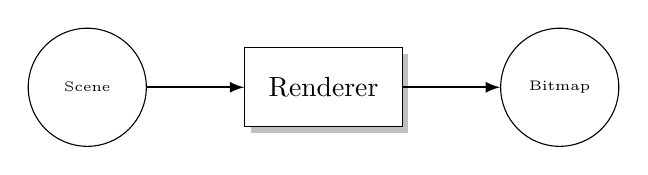
\begin{tikzpicture}[object/.style={draw,circle,font=\tiny,minimum size=1.5cm},pipeline/.style={draw,minimum width=2cm,minimum height=1cm,fill=white,drop shadow},arrow/.style={-latex,thick}]
  \node[pipeline] (renderer) {Renderer};
  \node[object] (scene) at ($ (renderer) + (-3, 0) $) {Scene};
  \node[object] (bitmap) at ($ (renderer) + (3, 0) $) {Bitmap};
  \draw[arrow] (scene) -- (renderer);
  \draw[arrow] (renderer) -- (bitmap);
\end{tikzpicture}

\end{document}